\subsection{Descripcion del problema}
El problema consiste en, dada:\\

-Una lista con $n$ pueblos, representados con sus pociciones $x$ e $y$ en el plano.\\

-Un numero $k$ que representa la cantidad maxima de centrales de gas a construir.\\

Conectar todos los pueblos a la red de gas construyendo centrales en a lo sumo pueblos y conectandolos por tuberias al resto de los pueblos, intentando minimizar el $riesgo$. donde el $riesgo$ es la distancia maxima de una tuberia construida entre dos pueblos.\\

Abstrayendonos del problema, podemos ver a los pueblos y tuberias como vertices y aristas de un grafo, y lo que queremos lograr es conseguir a lo sumo $k$ componentes conexas tales que el peso maximo entre todas las aristas sea minimo.

\subsubsection{Ejemplos}
Sea N el numero de pueblos, K la cantidad maxima de centrales, Pos:lista<ParXY> las posiciones de los pueblos en el plano, Q la cantidad de centrales construidas, M la cantidad de tuberias construidas, Centrales:lista<pueblos> los pueblos con centrales en ellos y Conexiones:lista<ParPueblo1Pueblo2> los vertices de las tuberias construidas (vease que una tuberia con vertices $x$ e $y$ es lo mismo que una tuberia con vertices $y$ y $x$).$\Rightarrow$
\begin{enumerate}
\item N: 1, K: 1, Pos:{(0,0)} \\
la respuesta es unica:
\begin{center}
  
   \begin{tabular}{| l | c | r | c | r | c | r | }
     \hline
     Q & M & Centrales & Conexiones \\ \hline
     1 & 0 & [1] & [ ]  \\
     \hline
   \end{tabular}
\end{center}

\item N: 2, K: 1, Pos:{(0,0),(0,1)} \\
las respuestas posibles son:
\begin{center}
  
   \begin{tabular}{| l | c | r | c | r | c | r | }
     \hline
     Q & M & Centrales & Conexiones \\ \hline
     1 & 1 & [1] & [(1,2)]  \\ \hline
     1 & 1 & [2] & [(1,2)] \\ 
     \hline
   \end{tabular}
 \end{center}
 
Vease que la central puede ubicarse tanto en un pueblo como en el otro.

\item N: 3, K: 2, Pos:{(0,0),(0,1),(8,8)} \\
las respuestas posibles son:
\begin{center}
  
   \begin{tabular}{| l | c | r | c | r | c | r | }
     \hline
     Q & M & Centrales & Conexiones \\ \hline
     1 & 1 & [1,3] & [(1,2)]  \\ \hline
     1 & 1 & [2,3] & [(1,2)] \\ 
     \hline
   \end{tabular}
 \end{center}
Como el pueblo agregado esta lejos de los otros y K=2 entonces tendra su propia central
\end{enumerate}

\subsection{Resolucion}
Para la resolucion de este problema lo primero que hicimos fue buscar como conectar todas los vertices como si solo tuvieramos una estacion, al hacerlo nos dimos cuenta de que podiamos usar prim sobre una tabla de adyacencias que tuviera todas las distancias entre pueblos. hacer prim nos servia, pues por el Lema 1, demostrado mas abajo, que dice que si minimizamos la suma de los pesos del arbol $\Rightarrow$ el peso maximo entre todas las aristas es minimo, tendriamos un arbol que cumplia que el peso maximo era minimo.
Luego teniamos que lograr esto para cuando hubiera mas de una estacion, asi llegamos al Lema 2, que dice que si a un arbol minimo le quitamos su mayor elemento $\Rightarrow$ las componentes conexas resultantes forman un bosque tal que el peso maximo entre todas las aristas sea minimo. asi que quitandole las k-1 aristas maximas al arbol minimo conceguiriamos un bosque de k componentes conexas que cumplian esta propiedad.
Finalmente faltaba ver donde poner las estaciones para que cada componente conexa del bosque tenga una y solo una estacion. vimos que poner la estacion en cualquier pueblo de una componente conexa no cambiaba las aristas del resultado. asi que recorrimos el bosque poniendo una estacion en cada componente conexa.

\subsubsection{Pseudocodigo}
\begin{algoritmo}{resolver}{\In{nPueblos}{Nat}, \In{kCentrales}{Nat}, \In{pueblos}{Lista<Coordenadas>}}
	Matrix tablaDistancias(nPueblos) \;
	tablaDistancias.llenarDistancias(nPueblos,pueblos) \;
	Lista(Par(Arista,double)) arbolMinimo \;
	Lista(Par(Arista,double)) bosqueMinimo \;
	\For{Nat \asignar 1 ; i $\leq$ nPueblos ; i++}{
		Nat j \asignar tablaDistancias.MinimoFila0()\;
		double distancia = tablaDistancias.DistanciaDe(0,j)\;
		Nat origen = tablaDistancias.OrigenDe(0,j)\;
		arbolMinimo.pushfront((origen,j),distancia)\;
		tablaDistancias.Combinar(j)
	}\;
	\If {kCentrales > nPueblos}{
		kCentrales = nPueblos\;
	}
	bosqueMinimo \asignar quitarKMasGrandes(arbolMinimo,kCentrales-1) \;
	Nat cantidadTuberias = bosqueMinimo.size() \;
	List(Nat) estaciones = generarEstaciones(bosqueMin,nPueblos) \;
	devolver(kCentrales, cantidadTuberias , estaciones, bosqueMinimo) \;
	
\end{algoritmo}

\subsection{Correctitud}
\subsubsection{Idea}
Sea $\Omega$ el grafo en el que los vertices representan los pueblos y las aristas las conexiones de gas posibles entre los pueblos con su riesgo, queremos demostrar que existe un arbol generador tal que el peso maximo entre las aristas es minimo. Como $\Omega$ es conexo, pues cada pueblo se conecta con todos los otros pueblos, sabemos que existe un $\Pi$ arbol generador minimo tal que se minimize la suma de los pesos del arbol. Por el Lema 1, como existe $\Pi$ puedo encontrar $\Pi'$ un arbol generador tal que el peso maximo entre las aristas es minimo.\\
luego queremos ver que quitarle aristas me devuelve un bosque correcto, por el Lema 2 cada vez que a un arbol de minimo maximo le quito su arista mas grande genero un bosque de minimo Maximo. Por lo tanto como quitamos las aristas mas grandes del bosque, y nunca sacamos mas que la cantidad de aristas que tiene el bosque, tenemos un bosque de minimo maximo. \\
Por ultimo queremos ver que genero una estacion y solo una en cada componente conexa del bosque, lo que hacemos es poner una en un vertice y recorrer todo el arbol del que es parte, y solo pongo estaciones en vertices que no recorri, cuando todos los vertices fueron recorridos se que hay una estacion en cada componente y se que es unica porque nunca recorro mas de una vez el mismo arbol.



\subsubsection{Lema 1: AGM $\Rightarrow$ peso maximo entre aristas minimo}
Sea $T$ un AGM del grafo $\Omega$, vease que:\\

$Peso(T) = \sum_{e \in T} Peso(e)$\\

$Peso(T) \leq Peso(T') \forall T'$ arbol generador de $\Omega$\\

llamo max(T) al maximo eje entre todos los ejes de T \\

Quiero ver que:\\

$Peso(T) \leq Peso(T') \forall T'$ arbol generador de $\Omega \Rightarrow$ max(T) $\leq$ max(T')\\

supongo que tengo un T' Arbol generador de G tal que max(T') < max(T) $\Rightarrow$ $\exists$ a arista, a $\in$ T, a $\notin$ T' que conecta dos vertices x e y, si sacaramos este vertice tendriamos dos componentes conexas que llamare A y B.\\

$\exists$ a' $\in$ T' / a' va de un nodo de A a un nodo de B (si este nodo no existiera T' no seria conexo). tomo:\\

T* = T - a + a'\\

$Peso(T$*$) = \sum_{e \in T} Peso(e) - Peso(a) + Peso(a')$\\

vease que $-Peso(a) + Peso(a') < 0$ pues a es algun maximo de T y todo a' en T' es menor que a, pues max(T') < max(T)\\

Por lo tanto: $Peso(T$*$) = \sum_{e \in T} Peso(e) - Peso(a) + Peso(a') < \sum_{e \in T} Peso(e) = Peso(T)$ ABSURDO!\\

el absurdo viene de suponer que max(T') < max(T) QED.

\subsubsection{Lema 2: AGM $\Rightarrow$ B = AGM - AristaMaxima es Bosque de minimos maximos}
Sea T un AGM de $\Omega$\\

B esta dividido en dos componentes conexas X e Y\\

Supongo que B = T - AristaMaxima no es Bosque de minimos maximos del grafo $\Omega$.\\

Sea G' un Grafo de minimos maximos del grafo $\Omega$ de dos componentes conexas, se que existe pues es tomar todos las aristas ordenadas y agregarle la arista minima hasta tener 2 componentes conexas, se que existe X' e Y' subarboles AGM de cada una de sus componentes conexas, pues para que halla un AGM en un grafo solo es necesario que sea conexo. llamo B' a X'+Y', que es un Bosque de minimos maximos de dos componentes conexas.\\

Se que existe en $\Omega$ una arista de peso minimo que une X' e Y', llamo a esta arista e'. $T'$ = X'+Y'+e' es un AGM de $\Omega$.\\

peso(T') = P(X')+P(Y')+P(e')\\

peso(T) = P(X)+P(Y)+P(AristaMaxima)\\

Vease que peso(T)=peso(T') pues ambos son AGM\\

si peso(e') $\leq$ peso(AristaMaxima) $\Rightarrow$ peso(X')+peso(Y') $\geq$ peso(X)+peso(Y) absurdo pues B es bosque minimo maximo y B' no\\

si peso(e') > peso(AristaMaxima) $\Rightarrow$ peso(X')+peso(Y') = peso(X)+peso(Y) absurdo T' no puede ser arbol minimo pues max(T') > max(T) 


\subsubsection{Conclusion}
Ahora sabemos que podemos encontrar un bosque de minimo maximo para cualquier conjunto de pueblos y podemos devolver un vertice de cada arbol del bosque.

\subsection{Complejidad}

\subsubsection{Introduccion}

Puede comprobarse en el c�digo que, omitiendo la carga de datos y las iteraciones requeridas
para manejar las distintas intancias del problema, el algoritmo ejecutado para la resoluci�n del problema es el siguiente.

Debajo del algoritmo se encuentran varias aclaraciones identificadas por el n�mero de l�nea.\\
\begin{algoritmo}{resolver}{\In{nPueblos}{Nat}, \In{kCentrales}{Nat}, \In{pueblos}{Lista<Coordenadas>}}
\LinesNumbered
\nl	
	Matrix tablaDistancias(nPueblos)\tcc*{$O$($n^2$)}
	tablaDistancias.llenarDistancias(nPueblos,pueblos) \tcc*{$O$($n^2$)}
	Lista(Par(Arista,double)) arbolMinimo \tcc*{$O$(1)}
	Lista(Par(Arista,double)) bosqueMinimo \tcc*{$O$(1)}
	\For(\tcc*[f]{$O$($n^2$)}){Nat i \asignar 1 ; i $\leq$ nPueblos ; i++}{
		Nat j \asignar tablaDistancias.MinimoFila0()\tcc*{$O$($n$)}
		double distancia = tablaDistancias.DistanciaDe(0,j)\tcc*{$O$(1)}
		Nat origen = tablaDistancias.OrigenDe(0,j)\tcc*{$O$(1)}
		arbolMinimo.pushfront((origen,j),distancia)\tcc*{$O$(1)}
		tablaDistancias.Combinar(j)\tcc*{$O$($n$)}
	}
	bosqueMinimo \asignar quitarKMasGrandes(arbolMinimo,kCentrales-1) \tcc*{$O$($nlog(n)$)}
	Nat cantidadTuberias = bosqueMinimo.size() \tcc*{$O$($n$)}
	Lista(Nat) estaciones = generarEstaciones(bosqueMin,nPueblos) \tcc*{$O$($n^2$)}
	devolver(kCentrales, cantidadTuberias , estaciones, bosqueMinimo) \tcc*{$O$($n$)}
	
\end{algoritmo}

\begin{algoritmo}{llenarDistancias}{\In{nPueblos}{Nat}, \In{pueblos}{Lista<Coordenadas>}}
\LinesNumbered
\setcounter{AlgoLine}{15}
\nl	
	Lista(Coordenada)::constiterator itI = pueblos.begin()\tcc*{$O$(1)}
	list(Coordenada)::constiterator itJ = pueblos.begin()\tcc*{$O$(1)}
	\For(\tcc*[f]{$O$($n^2$)}){Nat i \asignar 0; i != nPueblos ; i++}{
		double x1 = itI->first\tcc*{$O$(1)}
		double y1 = itI->second\tcc*{$O$(1)}
		\For(\tcc*[f]{$O$(n)}){Nat f \asignar 0; f != nPueblos ; f++}{
			double x2 = itJ->first\tcc*{$O$(1)}
			double y2 = itJ->second\tcc*{$O$(1)}
			double distancia = infinito\tcc*{$O$(1)}
			\If(\tcc*[f]{$O$(1)}){i != j}{
				distancia = sqrt((x1-x2)*(x1-x2) + ((y1-y2)*(y1-y2)))\tcc*{$O$(1)}
			}
			matriz[i][j].first = distancia\tcc*{$O$(1)}
			matriz[i][j].second = i+1\tcc*{$O$(1)}
			itJ++\tcc*{$O$(1)}
		}
		itI++\tcc*{$O$(1)}
		itJ = pueblos.begin()\tcc*{$O$(1)}
	}
	
\end{algoritmo}
\begin{algoritmo}{Combinar}{\In{fila}{Nat}}
\LinesNumbered
\setcounter{AlgoLine}{34}
\nl
	Nat dimension = Columnas()\tcc*{$O$(1)}
	double inf = infinito\tcc*{$O$(1)}
	matriz[0][fila].first = inf\tcc*{$O$(1)}
	\For(\tcc*[f]{$O$(n)}) {Nat j = 0 ; j != dimension ; j++}{
		Arista aristaF1 = makepair(0,j)\tcc*{$O$(1)}
		Arista aristaF2 = makepair(fila,j)\tcc*{$O$(1)}
		\If(\tcc*[f]{$O$(1)}){esfinito(DistanciaDe(aristaF1)) and DistanciaDe(aristaF2) $<$ DistanciaDe(aristaF1)}{
			matriz[0][j].first = DistanciaDe(aristaF2)\tcc*{$O$(1)}
			matriz[0][j].second = OrigenDe(aristaF2)\tcc*{$O$(1)}
		}
	}
\end{algoritmo}
\begin{algoritmo}{generarEstaciones}{\In{bosqueMinimo}{Lista(Par(Arista,double))},\In{nPueblos}{Nat}}[Lista(Nat)]
\LinesNumbered
\setcounter{AlgoLine}{45}
\nl
	Lista(Nat) res\tcc*{$O$(1)}
	vector(bool) yaLoVi (nPueblos, false)\tcc*{$O$(n)}
	vector(bool) conectados (nPueblos, false)\tcc*{$O$(n)}
	list(Nat) proximosVer\tcc*{$O$(1)}
	\For(\tcc*[f]{$O$(n)}){Nat i=0 ; i $<$ nPueblos ; i++}{
		proximosVer.pushback(i)\tcc*{$O$(1)}
	}
	\While(\tcc*[f]{$O$($n^2$)}){!proximosVer.empty()}{
		Nat sacar = proximosVer.front()\tcc*{$O$(1)}
		\uIf(\tcc*[f]{$O$(1)}){yaLoVi[sacar]}{
			proximosVer.popfront()\tcc*{$O$(1)}
		}\Else{
			\If(\tcc*[f]{$O$(1)}){!conectados[sacar]}{
				res.pushfront(sacar+1)\tcc*{$O$(1)}
			}
			proximosVer.popfront()\tcc*{$O$(1)}
			conectados[sacar] = true\tcc*{$O$(1)}
			yaLoVi[sacar] = true\tcc*{$O$(1)}
			lista(pair(Arista,double))::iterator itAM = bosqueMinimo.begin()\tcc*{$O$(1)}
			\While(\tcc*[f]{$O$($n$)}){itAM != bosqueMinimo.end() and bosqueMinimo.size() != 0}{
				\uIf {itAM-$>$first.first == sacar}{
					Nat j = itAM-$>$first.second\tcc*{$O$(1)}
					\If(\tcc*[f]{$O$($1$)}){!conectados[j]}{
						proximosVer.pushfront(j)\tcc*{$O$(1)}
						conectados[j] = true\tcc*{$O$(1)}
					}
					itAM = bosqueMinimo.erase(itAM)\tcc*{$O$(1)}
				}\textbf{else }\uIf(\tcc*[f]{$O$(1)}){itAM-$>$first.second == sacar}{
					Nat j = itAM-$>$first.first\tcc*{$O$(1)}
					\If(\tcc*[f]{$O$(1)}){!conectados[j]}{
						proximosVer.pushfront(j)\tcc*{$O$(1)}
						conectados[j]=true\tcc*{$O$(1)}
					}
					itAM = bosqueMinimo.erase(itAM)\tcc*{$O$(1)}
				}\Else{
					itAM++\tcc*{$O$(1)}
				}
			}
		}
	}
	return res\tcc*{$O$(n)}
\end{algoritmo}
\subsubsection{Aclaraciones del Pseudoc�digo}
1) inicializar una matriz vacia de tama�o nPueblos*nPueblos tarda $O$($n^2$)\\

2) Detallado entre las lineas 16 y 34,Llenar distancias toma cada pueblo y calcula su distancia con todos los demas, esto se logra en $O$($n^2$) iteraciones.\\

5) el while se corre n-1 veces, y adentro del while hay cosas que tardan $O$($n$), asi que la complejidad es $O$($n^2$).\\

6) buscar el minimo en un arreglo de n elementos desordenados tarda $O$($n$)\\

10) Detallado entre las lineas 35 y 45, lo que hace es combinar la fila 1 con la fila indicada, lo hace recorriendo las dos filas y guardando el minimo y su origen, recorrer de esta manera las dos filas es $O$($n$)\\

12) quitarKmasGrandes ordena el arbolMinimo de distancia de arista menor a distancia de arista mayor, ordenar cuesta $O$($nlog(n)$), luego de esto quita los k elementos mas grandes pasados como parametro, como como maximo puedo quitar las n aristas esto cuesta $O$($n$). por lo tanto la complejidad total es $O$($nlog(n)$)+$O$($n$)=$O$($nlog(n)$)\\

14) Detallado entre las lineas 46 y 86, generarEstaciones devuelve exactamente un nodo de cada componente conexa.\\

47) el vector yaLoVi sirve para saber si ya busque los adyacentes de un nodo alguna vez\\

48) el vector conectados sirve para agregar los adyacentes encontrados.\\

49) proximos ver es una lista en la cual se guardan los proximos nodos a los que se le buscaran adyacentes. antes de entrar al while lo inicializo con los pueblos de 1 a n.\\

53) la cantidad de veces maxima que se correra este while es 2n, pues puedo agregar pueblos al frente de la lista solamente si no se han agregado antes, o sea si en el vector conectados estaba en false su posicion. o sea que como maximo agregare todos los pueblos al frente de la lista y cada pueblo estara dos veces en la lista, pero me aseguro de no correr la busqueda de adyacentes de un nodo que ya vi con el vector yaLoVi. como este while se corre $O$($n$) veces, y adentro hay algo que se corre $O$($n$) veces cada vez que se llama el algoritmo, entonces es $O$($n^�$)

\subsubsection{Conclusion}

Como este algoritmo es iterativo, o sea no tiene partes recursivas, la complejidad total es la suma de las complejidades, luego si sumamos las complejidades de cada linea obtenemos que este algoritmo es O($n^2$), siendo n la cantidad de pueblos del mapa. ademas, como la cantidad de centrales siempre se puede acotar por la cantidad de pueblos (una central por pueblo) en los puntos en los que la complejidad depende de la cantidad de centrales siempre la podemos acotar por la cantidad de pueblos.

\subsection{Testing}
Los casos bordes que consideramos en este ejercicio son los que:
\begin{enumerate}
\item tienen muchos pueblos en un solo lugar
\item tienen tres pueblos que estan a distancias iguales entre ellos
\item tienen mas pueblos que estaciones
\item tienen pueblos en los cuadrantes positivos y negativos del mapa

\end{enumerate}
\begin{center}
  \begin{tabular}{| l | c | r | c | r |c | r | }
    \hline
     Numero Estaciones & Pueblos & Estaciones construidas & Conexiones construidas \\ \hline
     2 & [(1,1),(1,1),(1,1)] & [1,2] & [(3,1)] \\ \hline
     2 & [(0,0),(0,10),($\sqrt{10^2-5^2}$,5)] & [1,2] & [(3,2)] \\ \hline
     100 & [(1,1),(2,2),(2,2)] & [1,2,3] & [ ] \\ \hline
     2 & [(1,1),(1,-1),(-1,1),(-1,-1)] & [1,2] & [(4,2),(3,1)] \\ 
     \hline
   \end{tabular}
 \end{center}
\paragraph{Nota}
La validez de estos resultados se comprobo a mano, mas no se adjuntan las cuentas pues creemos que no aportan mucho mas que espacio malgastado. (Salvemos un arbol! Ahorremos papel!)

\subsection{Experimentaci�n}
Para la experimentaci�n, generamos instancias aleatorias de distintos tama�os, variando la cantidad de centrales. Siendo n el tama�o de
la entrada. L�ase por aleatoria, creada por la funci�n Rand() de C++ y manipulada lo m�nimamente necesario para que diera un numero razonable.
La manipulaci�n se muestra en el Anexo del c�digo, en la parte correspondiente al archivo $ejemplos\_random.cpp$.

\paragraph{Gr�fico 1}
Para este gr�fico usamos generamos mapas con centrales = 1, centrales = numero de pueblos y centrales= aleatorias entre 1 y el numero de pueblos.
muestra el tiempo, en microsegundos, requerido para resolver el problema.

\begin{figure}[H]
    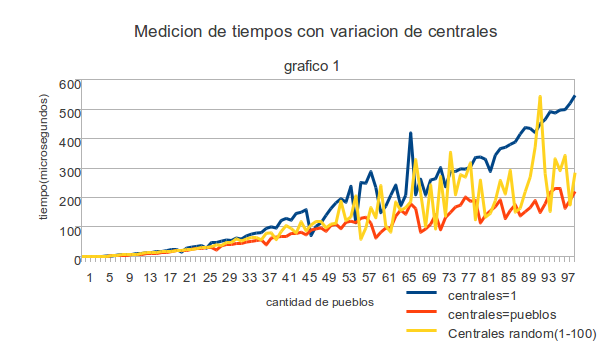
\includegraphics[width=0.8\textwidth]{grafico2-1.png}
  \label{fig:ejemplo}
\end{figure}

\paragraph{Gr�fico 2}
Para este gr�fico lo que hacemos es $constantizar$ el gr�fico 1, es decir, dividimos las mediciones 
por la complejidad que calculamos, en este caso $n^2$. \\

\begin{figure}[H]
    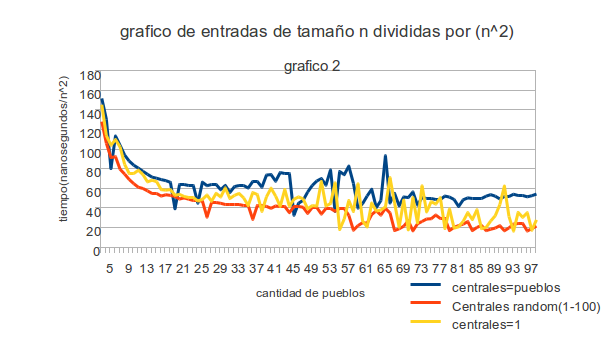
\includegraphics[width=0.8\textwidth]{grafico2-2.png}
  \label{fig:ejemplo}
\end{figure}

\subsubsection{Conclusiones} 
\paragraph{Gr�fico 1}
En este gr�fico se ven los dos casos extremos de C1:centrales = 1 y CN:centrales = numero de pueblos, se ve que claramente C1 es un peor caso y CN es un mejor caso, y que CR:centrales= (aleatorias entre 1 y el numero de pueblos)  oscila entre estos dos casos. esto muestra que la cantidad de centrales afecta al tiempo de computo del algoritmo, si bien esta acotada por el peor caso.

\paragraph{Gr�fico 2}
Queremos hacer notar que el gr�fico tiende a una constante, es decir, que efectivamente la complejidad es la esperada. para esto constantizamos los tres casos vistos en el grafico 1 para que se vea que la complejidad en peor y mejor caso queda constante al ser dividida por $n^2$ y que todos los otros casos oscilan entre estas dos constantes. \\
